\documentclass[11pt]{article}
\usepackage[T1]{fontenc}
\usepackage[utf8]{inputenc}
\usepackage[]{babel}
\usepackage{tikz}
\usepackage{pgfplots}
\usepackage{graphicx}
\usepackage{float}
\usepackage{amssymb}
\usepackage{amsmath}
\title{Algorytmy Metaheurystyczne}
\author{Szymon Brzeziński - 254611 \\
Paweł Prusisz - 254642}
\date{05.12.2021}
\begin{document}
\maketitle


\section{Opis}
    Tematem pracy jest przetestowanie oraz opis algorytmu Tabu Search rozwiązującego instancje problemu komiwojażera.
    \\Badane instancje są wczytywane z biblioteki TSPLIB oraz generowane losowo.
    \\Typy instancji:
    \begin{enumerate}
        \item Symetryczne
        \item Asymetryczne
        \item Euklidesowe
    \end{enumerate}
    Badane algorytmy:
    \begin{enumerate}
        \item extended nearest neighbour
        \item two-opt
        \item tabu-search
    \end{enumerate}

\section{Jakość rozwiązań}
    Pierwszą badaną zależnością jest porównanie rozwiązań zwróconych przez
    tabu searchwzględem rozmiaru problemu w stosunku do wczesniej zaimplementowanych algorytmów. 
    W tym celu dla każdego badanego rozmiaru n zostały wygenerowane 10 różnych instancji na których wywołano 
    algorytmy nearest neighbour extended, two-opt oraz tabu search. 
    Ilość iteracji dla tabu jest równa wielkości problemu.
    Długość zwróconej ścieżki oraz czas działania algorytmów został uśredniony dla każdego n

    \subsection{Wykresy}

    \subsubsection{Instacja Symetryczna}
    \begin{center}
        \begin{figure}[H]
            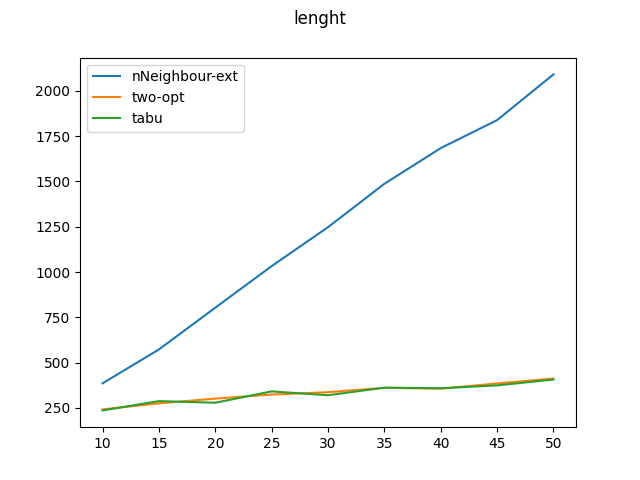
\includegraphics[scale=0.50]{symetricLen.png}
        \end{figure}
    \end{center}
    \begin{center}
        \begin{figure}[H]
            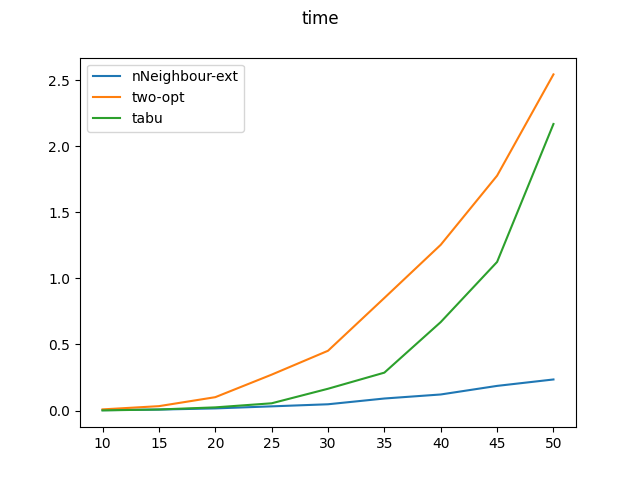
\includegraphics[scale=0.50]{symetricTime.png}\\
        \end{figure}
    \end{center}
        
    \subsubsection{Instacja Asymetryczna}
    \begin{center}
        \begin{figure}[H]
            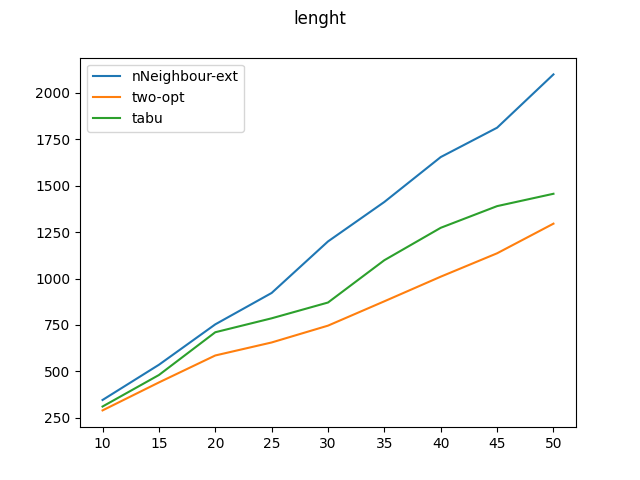
\includegraphics[scale=0.50]{asymetricLen.png}
        \end{figure}
    \end{center}
    \begin{center}
        \begin{figure}[H]
            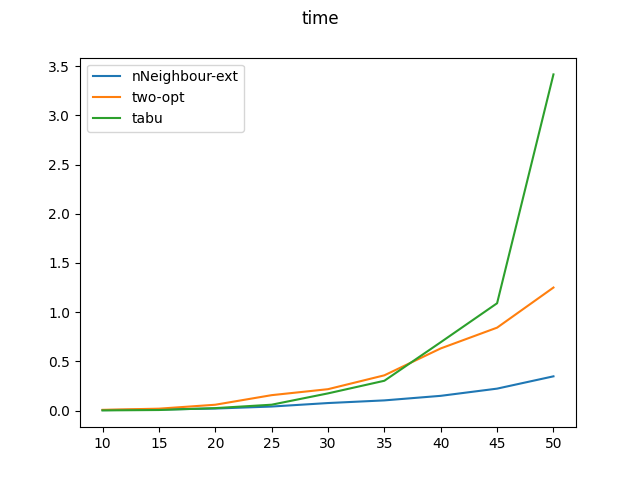
\includegraphics[scale=0.50]{asymetricTime.png}\\
        \end{figure}
    \end{center}

    \subsubsection{Instacja Euklidesowa}
    \begin{center}
        \begin{figure}[H]
            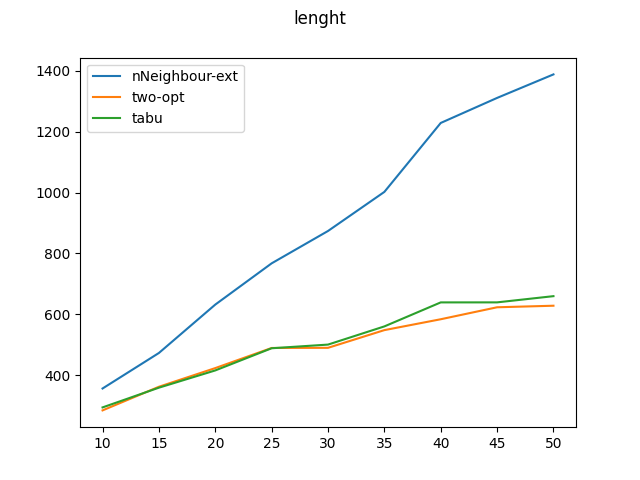
\includegraphics[scale=0.50]{euc2dLen.png}
        \end{figure}
    \end{center}
    \begin{center}
        \begin{figure}[H]
            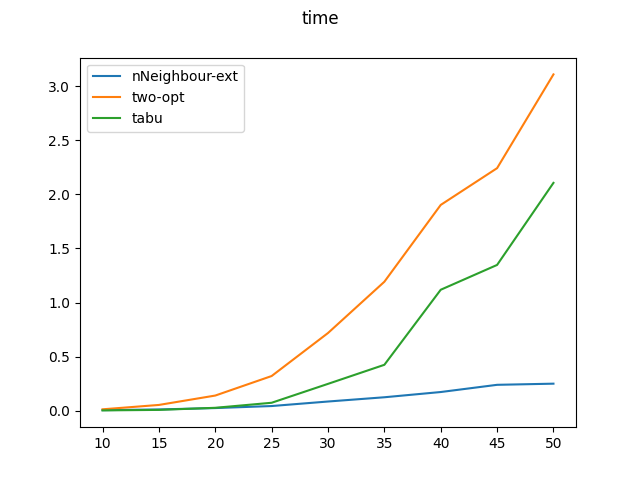
\includegraphics[scale=0.50]{euc2dTime.png}\\
        \end{figure}
    \end{center}

    \subsection{Wnioski }   
    Z uzyskanych wyników mżemy zobaczyć iż tabu search dla danych wywołań zwraca podobne wyniki 
    jak algorytm two-opt. Czasowo tabu search wypadł bardzo podobnie do algorytmu two-opt, jednak
    wynika to z możliwości manualnego sterowania iloscia iteracji. 







\section{Jakość rozwiązań w tym samym czasie }
        Tym razem zbadany jak poradzi sobie tabu search przy ograniczonym czasie działania.
        Testy wykoywane były następujący sposób: dla danej losowej instancji uruchamiany był algorytm
        nearest neighbour extended, jego czasdziałania był ograniczeniem czasowym dla pozostałych 2
        algorytmów. Wyniki tego testu prezentują się nastepująco.
    \subsection{Wykresy }
        \subsubsection{Instancja Symetryczna }
                \begin{center}
                \begin{figure}[H]

                    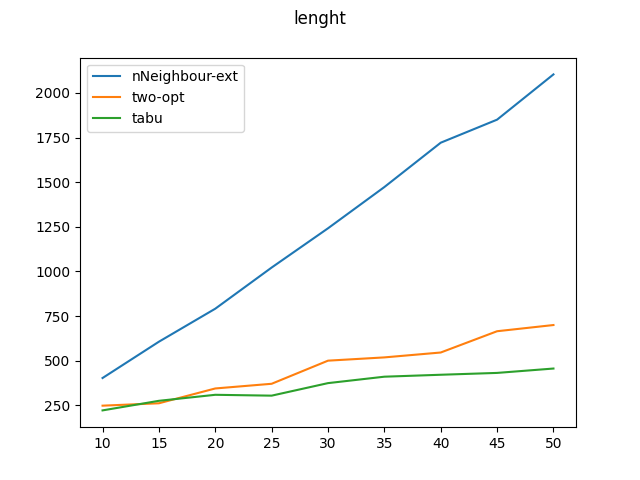
\includegraphics[scale=0.6]{timedSymetricLenght.png}

                \end{figure}
                \end{center}

        \subsubsection{Instancja Asymetryczna }
                \begin{center}
                \begin{figure}[H]

                    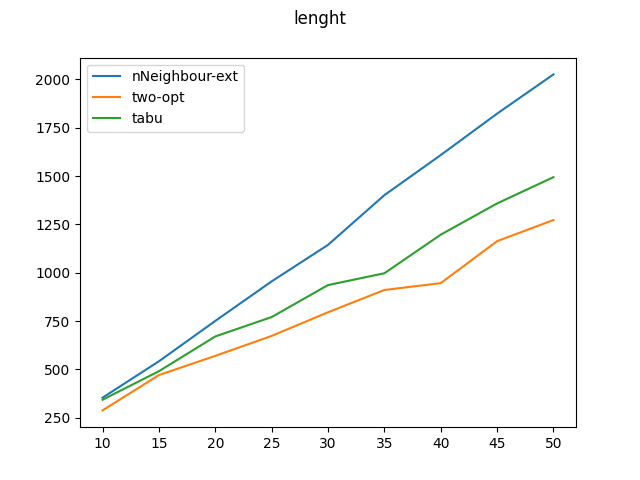
\includegraphics[scale=0.6]{timedAsymetricLenght.png}

                \end{figure}
                \end{center}
        \subsubsection{Instancja Euklidesowa }
                \begin{center}
                \begin{figure}[H]

                    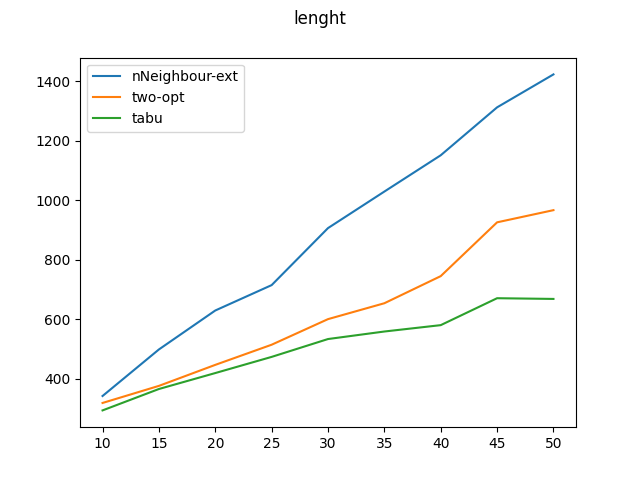
\includegraphics[scale=0.6]{timedEuc2dLenght.png}

                \end{figure}
                \end{center}
    \subsection{Wnioski }
        W przypadku instancji asymetrycznej tabu search ogazał się goszy od algorytmu two-opt, 
        a dla pozostałych przypadków udało mu się znaleźć lepszą scieżkę przy tym samym ograniczeniu czasowym.


\section{Porównanie z optymalnym }
    W tym badaniu sprawdzimy jak prezentują się wyniki tabu search w porównaniu do rozwiązania optymalnego
    \subsection{Wykresy}
        \subsubsection{Berlin52}
            \begin{center}
            \begin{figure}[H]

                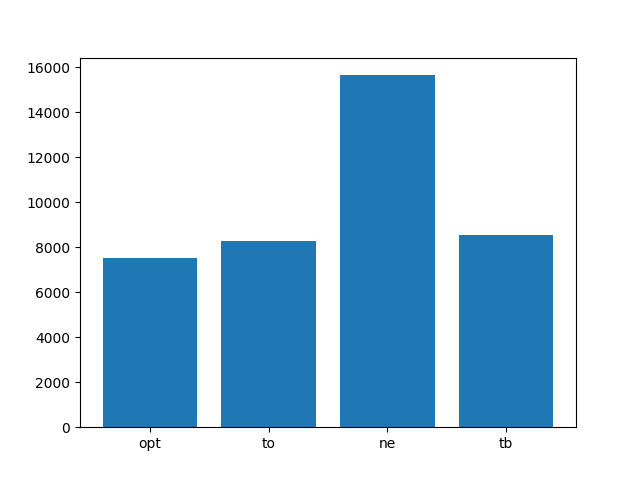
\includegraphics[scale=0.6]{berlin52.png}

            \end{figure}
            \end{center}

        \subsubsection{att48}
            \begin{center}
            \begin{figure}[H]

                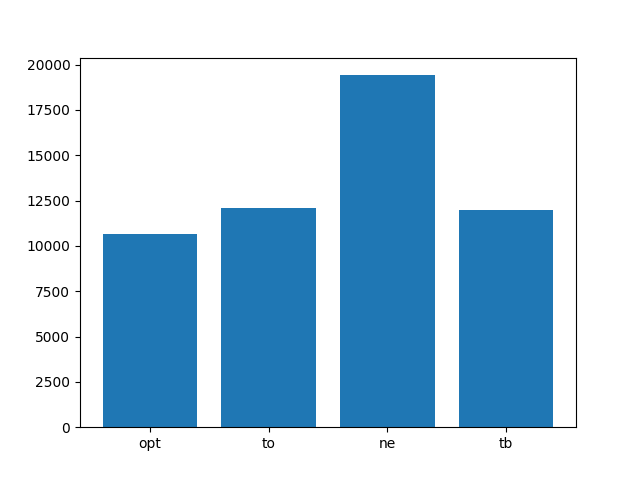
\includegraphics[scale=0.6]{att48.png}

            \end{figure}
            \end{center}

        \subsubsection{ulysses22}
            \begin{center}
            \begin{figure}[H]

                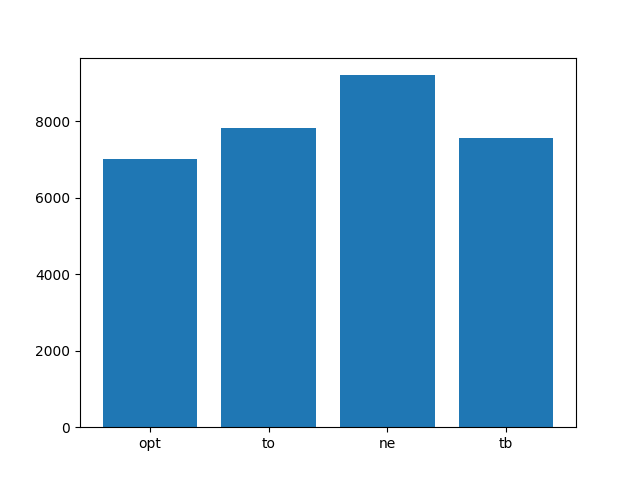
\includegraphics[scale=0.6]{ulysses22.png}

            \end{figure}
            \end{center}

    \subsection{Wnioski}
        Tabu search dla wszytkich testowanych przypadków zwrócił wynik najbliższy optymalnego 
        spośród testowanych algorytmów.

\section{Wielkość listy tabu}
        W tym badaniu sprawdzimy jak wielkość listy tabu wpływa na wynik.
        Testowane dla 2 instancji, ulysses22 oraz ulysses16 wielkość listy tabu zmieniała sie od
        1 do 50. Na wykresach przedstawiono długość znalezionego rozwiązania w zależności od 
        długości listy tabu

        \subsection{Wykresy}
            \subsubsection{Ulysses22}
                \begin{center}
                \begin{figure}[H]

                    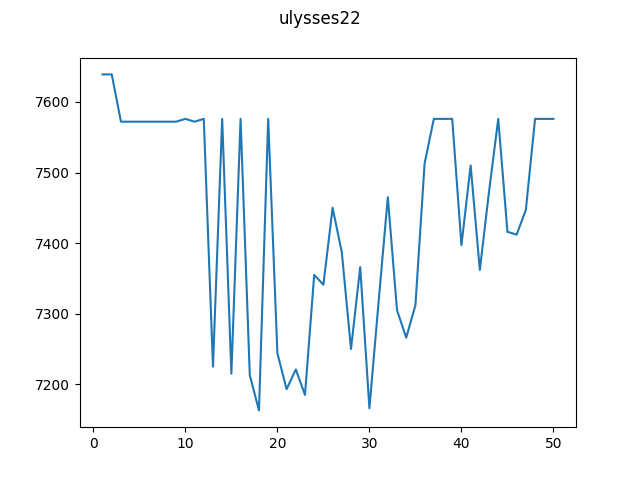
\includegraphics[scale=0.6]{tabuListUlysses22.png}

                \end{figure}
                \end{center}

            \subsubsection{Ulysses16}
                \begin{center}
                \begin{figure}[H]

                    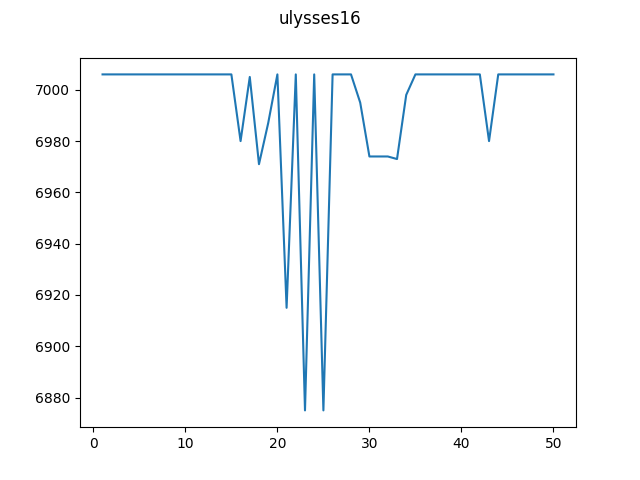
\includegraphics[scale=0.6]{tabuListUlysses16.png}

                \end{figure}
                \end{center}
    \subsection{Wnioski}
        Jak widać na wykresach długość listy tabu wpływa na jakość rozwiązania. Dla instancji Ulysses22
        długość listy 30 dała najlepszy rezultat, natomiast w przypadku instancji Ulysses16 najlepszy
        wynik otrzymano dla długości 23 i 25.
\end{document}